\documentclass[runningheads]{llncs}

\usepackage{amsmath}
\usepackage{booktabs}
\usepackage{flafter}
\usepackage{graphicx}
\usepackage{microtype}
\usepackage{url}

\begin{document}

\title{GARCH--Autoformer: Hybrid Residual Correction under
Multi-Distribution Accuracy--Risk Evaluation}
\titlerunning{GARCH--Autoformer under Multi-Distribution Risk Evaluation}

\author{Anonymous Author(s)}
\authorrunning{Anonymous Author(s)}
\institute{Anonymous institution for double-blind review}

\maketitle

\begin{abstract}
Volatility forecasting must preserve point accuracy while supporting
calibrated tail-risk decisions. We propose GARCH--Autoformer, a hybrid
residual-correction architecture that combines a structured
GJR--GARCH variance path with a decomposition encoder operating on
standardized innovations. Positive variance fusion retains the
econometric baseline while allowing nonlinear multi-horizon
corrections. Risk is reconstructed independently with Normal,
Student-\(t\), and filtered-historical-simulation VaR; method-level
backtest criteria are averaged before SAW and TOPSIS ranking. The study
contains 1,322,330 predictions from 26 configurations, nine equity
markets, and five horizons. Under this primary multi-distribution
definition, MoiraiVaR--Moirai-MoE ranks first under both 50:50 and
30:70 accuracy--risk policies. GARCH--Autoformer Tier~2 ranks twelfth
under both policies, although it ranks first when risk is measured by
Student-\(t\) VaR alone. The result identifies a distribution-specific
strength rather than distribution-robust superiority and shows why a
single VaR assumption can materially change architectural conclusions.

\keywords{GARCH--Autoformer; volatility forecasting; Value-at-Risk;
hybrid architecture; multi-criteria decision making}
\end{abstract}

\section{Introduction}

Volatility is latent, persistent, and operationally linked to market
risk. ARCH and GARCH provide interpretable conditional-variance
dynamics~\cite{engle1982,bollerslev1986}; the asymmetric GJR extension
also represents leverage effects~\cite{glosten1993}. Deep sequence
models can learn richer temporal patterns, but a lower point loss does
not by itself imply realistic volatility amplitude or calibrated
Value-at-Risk (VaR). Rankings also depend on the target, proxy, and
loss~\cite{patton2011}. A useful architecture should therefore improve
flexibility without discarding the inductive structure needed for risk.

We introduce \emph{GARCH--Autoformer}, a hybrid architecture designed
around that requirement. GJR--GARCH supplies a recursive variance path.
A decomposition encoder inspired by Autoformer receives standardized
innovations and predicts a horizon-wise variance correction. The two
branches are fused in variance space with a positive link. Training uses
a Student-\(t\) likelihood, connecting the learned scale to heavy-tailed
returns rather than only to a volatility proxy.

The paper makes three contributions. First, it specifies the new hybrid
residual-correction design and two capacity tiers. Second, it evaluates
the intended accuracy--risk balance with five forecast/dynamics
criteria and four risk criteria averaged across three VaR
constructions, rather than selecting on one error or one return
distribution. Third, it isolates the scope of the architectural claim:
GARCH--Autoformer is preferred under Student-\(t\) VaR alone, but not
under the distribution-averaged primary analysis. This reversal is
itself evidence that model-selection claims must report their VaR
construction.

\section{Related Work}

GARCH remains a demanding benchmark even against richer econometric
specifications~\cite{hansen2005}; FIGARCH extends this line to
long-memory dynamics~\cite{baillie1996}. Neural hybrids later combined
GARCH structure with recurrent networks~\cite{zhao2024}, while
Multi-Transformer--GARCH joined attention and econometric features
~\cite{mishra2024}. Our design instead learns a signed, horizon-wise
correction to a recursive GJR--GARCH path and fuses both branches
directly in variance space.

The Transformer~\cite{vaswani2017}, Reformer~\cite{kitaev2020}, and
Informer~\cite{informer2021} provide relevant attention baselines.
Autoformer introduced progressive decomposition~\cite{wu2021};
FEDformer moved decomposition into Fourier/Wavelet representations
~\cite{fedformer2022}. Moirai and Moirai-MoE provide pretrained
alternatives~\cite{woo2024,liu2025}. Because simple linear models can
outperform complex Transformers~\cite{zeng2023}, our evaluation rejects
degenerate low-dynamics forecasts before ranking.

Parametric Normal VaR is the classical variance--covariance baseline
popularized by RiskMetrics~\cite{riskmetrics1996}. Conditionally
Student-\(t\) innovations represent heavier return tails
~\cite{bollerslev1987}, while filtered historical simulation (FHS)
combines volatility filtering with an empirical innovation
distribution~\cite{baroneadesi1999}. We retain all three because each
imposes a different tail shape; the primary risk score averages their
diagnostics rather than allowing one distribution to determine the
ranking.

SAW follows additive-utility aggregation~\cite{triantaphyllou2000},
whereas TOPSIS uses distance from ideal and anti-ideal solutions
~\cite{hwang1981,behzadian2012}. Reporting both exposes sensitivity to
normalization and compensation.

\section{Proposed GARCH--Autoformer}

\subsection{Structured and learned branches}

For returns \(r_t=\sigma_t z_t\), the GJR--GARCH branch estimates
\[
\sigma^2_{G,t}=\omega+\alpha\epsilon^2_{t-1}
+\gamma\mathbf{1}(\epsilon_{t-1}<0)\epsilon^2_{t-1}
+\beta\sigma^2_{G,t-1}.
\]
Parameters are fitted on the training split and recursively produce the
base path \(\sigma^2_{G,t+1:t+H}\). This branch gives persistence,
asymmetry, and a stable scale prior.

The learned branch uses the last \(L=60\) standardized innovations
\(z_{t-L+1:t}=r/\sigma_G\). After within-window scaling, a linear
embedding and positional encoding, stacked decomposition blocks separate
local trend and residual information. A feed-forward residual head maps
the flattened representation to
\(\Delta_{1:H}\). Tier~1 uses \(d=32\), two encoder layers, and
\(d_{\rm ff}=128\); Tier~2 uses \(d=128\), three layers, and
\(d_{\rm ff}=512\).

\begin{figure}[t]
\centering
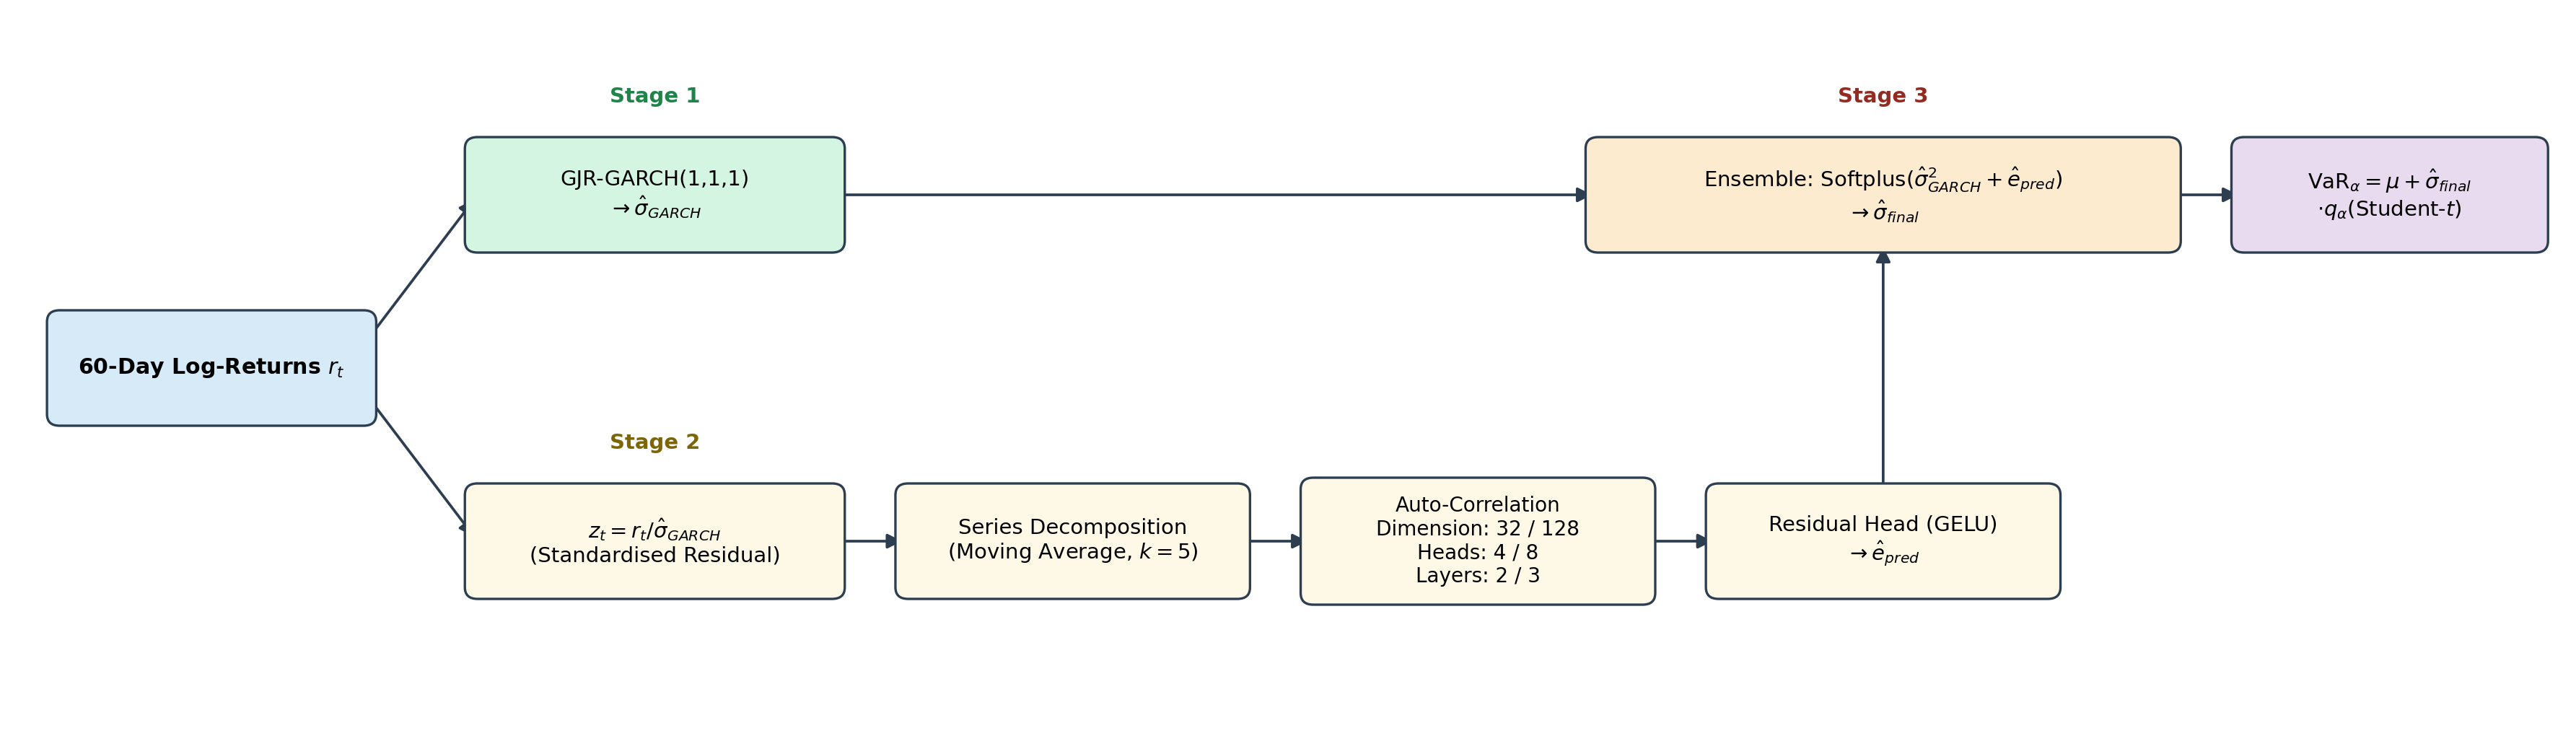
\includegraphics[width=\textwidth]{fig_garch_autoformer_architecture}
\caption{GARCH--Autoformer. A structured GJR--GARCH variance path and a
learned innovation correction meet in positive variance fusion.}
\label{fig:architecture}
\end{figure}

\subsection{Positive residual fusion and objective}

As shown in Fig.~\ref{fig:architecture}, the hybrid output is
\[
\hat\sigma_{t+h}=
\sqrt{\operatorname{softplus}\!\left(
\sigma^2_{G,t+h}+\Delta_h\right)},\quad h=1,\ldots,H .
\]
Predicting a correction instead of a complete volatility path anchors
the network to an econometric baseline; allowing signed
\(\Delta_h\) lets it raise or lower that baseline. Softplus guarantees a
positive final variance. With training-split degrees of freedom \(\nu\),
parameters minimize the zero-mean Student-\(t\) negative log-likelihood
\[
\mathcal{L}=\frac{1}{nH}\sum_{i,h}\left[
\log\hat\sigma_{i,h}+
\frac{\nu+1}{2}\log\left(1+
\frac{r_{i,h}^{2}}{\nu\hat\sigma_{i,h}^{2}}\right)\right].
\]
This construction targets an accuracy--risk balance in two ways:
nonlinear residual correction supplies forecast flexibility, while the
GARCH path, positive scale, and heavy-tailed likelihood preserve a
risk-compatible representation. The empirical protocol below tests
whether that design goal is realized.

\section{Accuracy--Risk Evaluation}

\subsection{Three VaR constructions}

For \(\alpha\in\{0.01,0.05\}\), zero conditional mean, predicted scale
\(\hat\sigma_t\), Normal quantile \(z_\alpha\), and Student-\(t\)
quantile \(t_{\alpha,\nu}\), the first two left-tail thresholds are
\[
\widehat{\mathrm{VaR}}^{N}_{\alpha,t}
=\hat\sigma_tz_\alpha,\qquad
\widehat{\mathrm{VaR}}^{t}_{\alpha,t}
=\hat\sigma_tt_{\alpha,\hat\nu}.
\]
Normal VaR follows the parametric RiskMetrics convention
~\cite{riskmetrics1996}. The Student-\(t\) degrees of freedom are fitted
per market and bounded below by 2.1; the construction follows the
heavy-tailed conditional model of Bollerslev~\cite{bollerslev1987}.
For FHS, standardized residuals are
\(u_s=r_s/\hat\sigma_s\), and
\[
\widehat{\mathrm{VaR}}^{FHS}_{\alpha,t}
=\hat\sigma_t\widehat Q_\alpha
\{u_{t-250},\ldots,u_{t-1}\}.
\]
The one-step shift makes the threshold depend only on past residuals.
This is the volatility-filtered empirical-quantile principle of
Barone-Adesi et al.~\cite{baroneadesi1999}. A violation occurs when
\(r_t<\widehat{\mathrm{VaR}}_{\alpha,t}^{m}\).

Each method \(m\in\{N,t,FHS\}\) is backtested separately in every
market--horizon block. Let \(PR_{\alpha,m}\) be the proportion of blocks
passing both Kupiec coverage~\cite{kupiec1995} and Christoffersen
independence~\cite{christoffersen1998}, and let
\(E_{\alpha,m}=|\bar p_{\alpha,m}-\alpha|\), where
\(\bar p_{\alpha,m}\) is the equally weighted mean block violation
rate. The MCDM risk inputs are
\[
\overline{PR}_{\alpha}=\frac{1}{3}\sum_m PR_{\alpha,m},
\qquad
\overline E_{\alpha}=\frac{1}{3}\sum_m E_{\alpha,m}.
\]
Thus ``VaR 1\%'' and ``VaR 5\%'' in the primary ranking denote means of
method-level diagnostics. The three numerical VaR thresholds are not
averaged.

\subsection{Forecast criteria and Sanity Gate}

Let \(y_i>0\) and \(\hat y_i>0\) be observed and predicted volatility.
Scoring rules must match the forecast target~\cite{gneiting2011}; we use
MSE, MAE, and QLIKE as complementary point losses, where
\[
\mathrm{QLIKE}=\frac1n\sum_i\left(
\frac{y_i}{\hat y_i}-\log\frac{y_i}{\hat y_i}-1\right).
\]
Dynamics are represented by amplitude error
\(e_\sigma=|s_{\hat y}/s_y-1|\) and tracking error
\(e_\rho=1-\max(\rho(y,\hat y),0)\). Together with
\(\overline{PR}_{.01}\), \(\overline E_{.01}\),
\(\overline{PR}_{.05}\), and \(\overline E_{.05}\), the decision matrix
contains nine criteria.

A configuration is eligible only when every criterion is finite,
\(e_\sigma\leq0.9\), and mean tracking correlation is positive. This
Sanity Gate prevents a nearly constant forecast from compensating for
missing dynamics through unrelated risk criteria.

\subsection{Decision policies and statistical analysis}

Simple Additive Weighting (SAW)~\cite{triantaphyllou2000} applies
benefit/cost min--max normalization and sums weighted scores. TOPSIS uses
vector normalization and ranks closeness to the weighted ideal
~\cite{hwang1981,behzadian2012}. Their ordinal ranks are averaged; lower
consensus rank is better. The balanced policy allocates 50\% to
forecast/dynamics and 50\% to VaR. The risk-priority policy allocates
30:70. Criteria receive equal weight within each group; method
averaging occurs before SAW/TOPSIS normalization.

\begin{figure}[t]
\centering
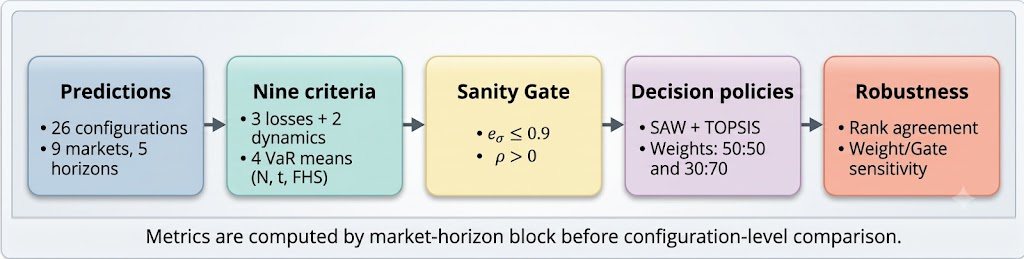
\includegraphics[width=.98\textwidth]{fig_evaluation_pipeline}
\caption{Experimental evaluation under explicit accuracy--risk
preferences. Each VaR criterion first averages Normal, Student-\(t\),
and FHS diagnostics.}
\label{fig:pipeline}
\end{figure}

Figure~\ref{fig:pipeline} summarizes the evaluation. Metrics are first
computed for each of 45 market--horizon blocks and then aggregated by
configuration. Forecast-loss differences are assessed with the Friedman
test and Kendall's \(W\), following block-wise comparison
guidance~\cite{demsar2006}. Rank agreement, weight sweeps, and Gate
sweeps test whether the conclusion depends on one decision setting.

\section{Experimental Study}

\subsection{Data and competitors}

The experiment contains 1,322,330 daily predictions for VN-Index,
VN30, KOSPI, Nikkei~225, DAX~40, Euronext~100, IBEX~35, SMI, and
S\&P~500 at horizons \(\{1,3,5,10,21\}\). The 26 configurations include
four GARCH variants, including FI-GARCH~\cite{baillie1996} and
GARCH--LSTM~\cite{zhao2024}; twelve Autoformer, Informer, Reformer, and
vanilla-Transformer tiers~\cite{wu2021,informer2021,kitaev2020,vaswani2017};
three Moirai-family models~\cite{woo2024,liu2025}; three VaR-aware
variants; and four GARCH-/Wavelet--Autoformer hybrids.
Autoformer is included because its decomposition principle is directly
related to the learned branch~\cite{wu2021}; linear and foundation-model
results in prior work motivate heterogeneous comparators
~\cite{zeng2023,woo2024}.

\subsection{Implementation details}

Splits are chronological and market specific. Within GARCH--Autoformer,
GJR--GARCH parameters and likelihood degrees of freedom are estimated
on training observations. The post-hoc Student-\(t\) VaR evaluator
fits one degree-of-freedom parameter per market; FHS uses a shifted
250-observation window. Both tiers use a 60-day input and produce 21
steps; reported horizons select steps 1, 3, 5, 10, and 21. Training uses AdamW
(\(10^{-3}\), weight decay \(10^{-4}\)), batch size 128, at most 30
epochs, gradient clipping at 1, and validation-likelihood early stopping
with patience 5.

\subsection{Main rankings}

The Gate retains 21 configurations and excludes five for excessive
amplitude error, non-positive tracking, or both. Figure~\ref{fig:ranks}
shows the leading ranks.

\begin{figure}[t]
\centering
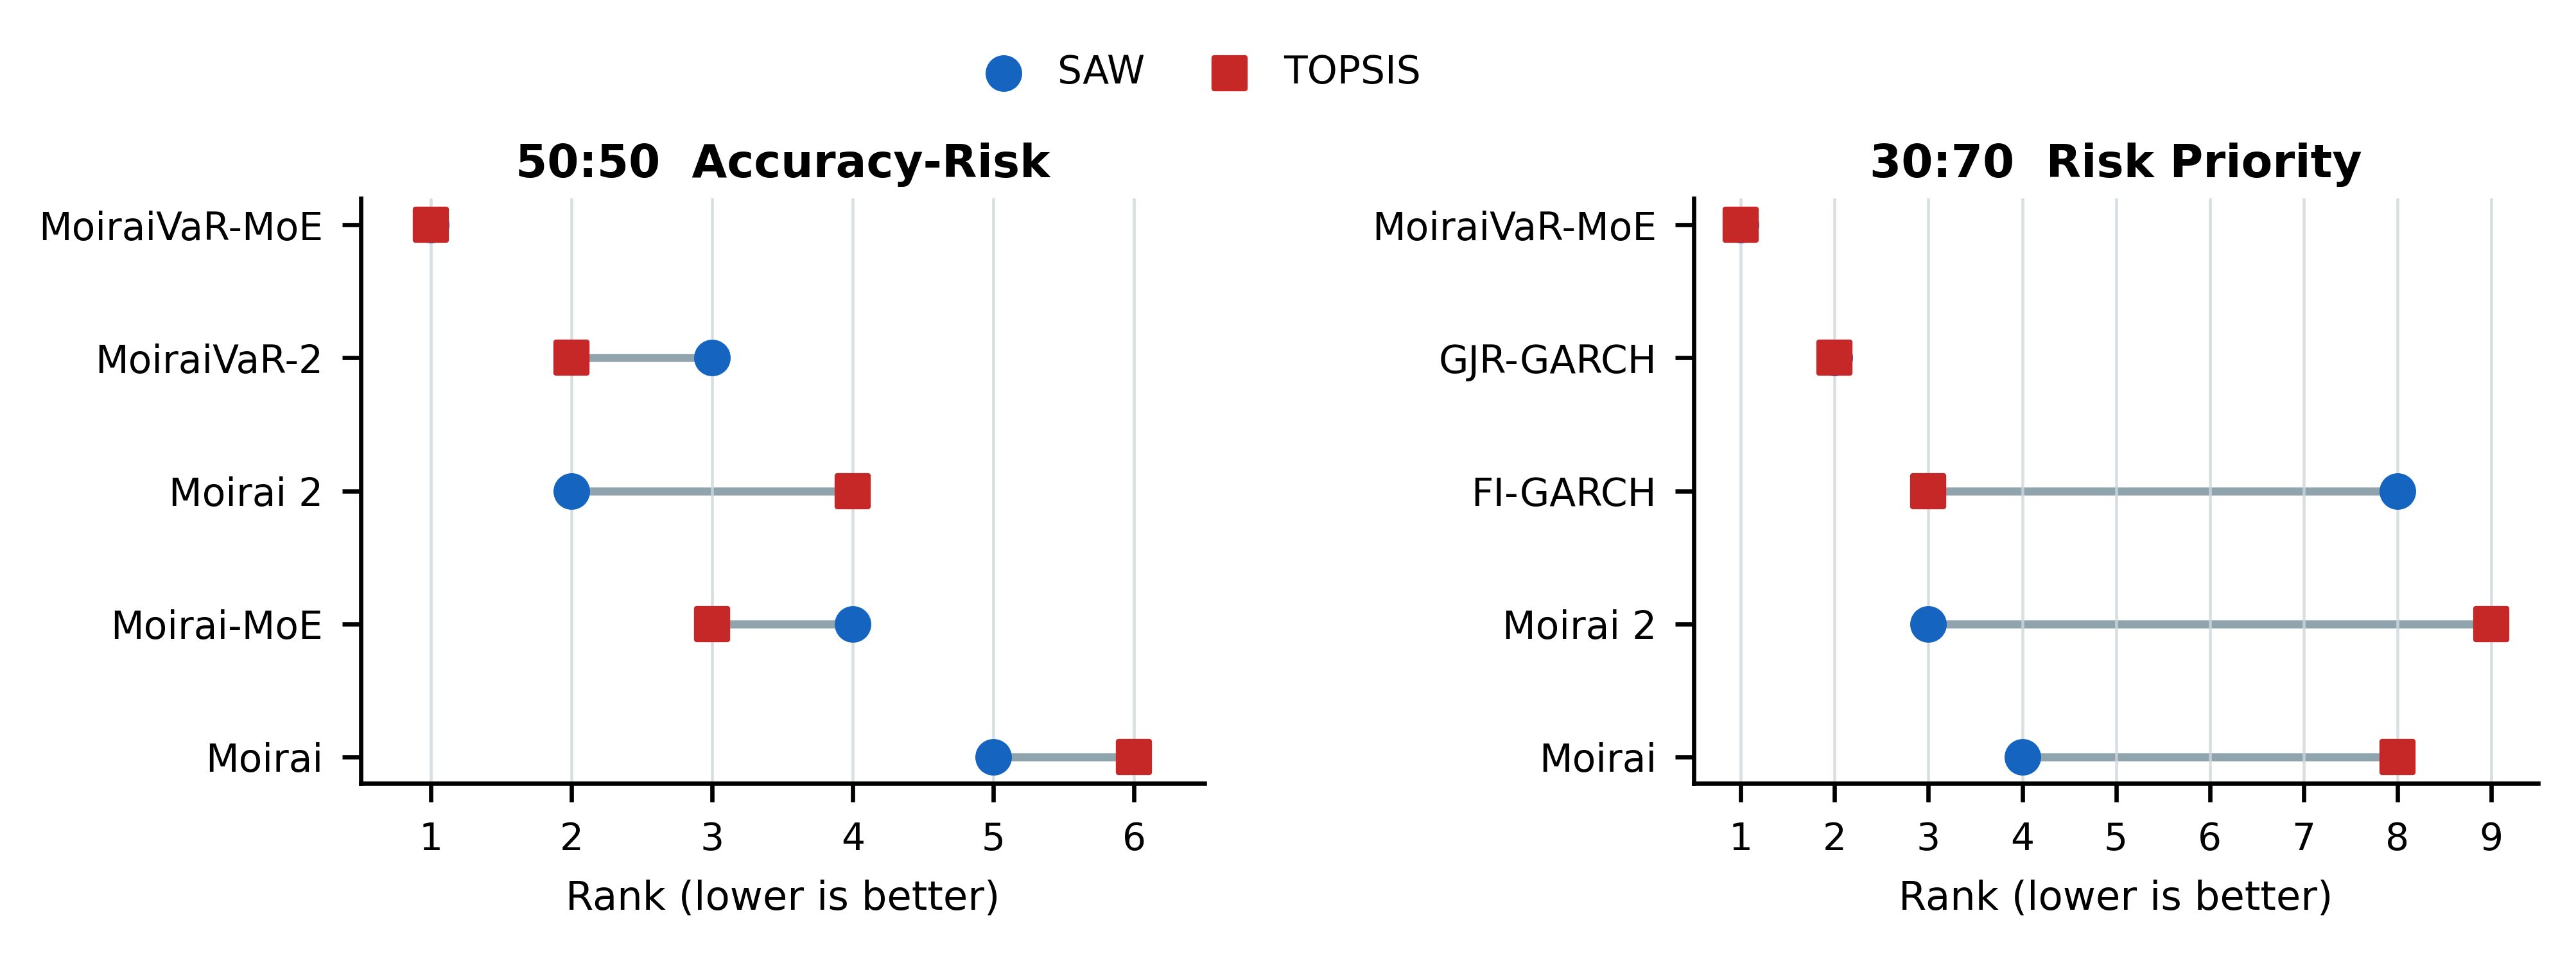
\includegraphics[width=\textwidth]{fig_rank_comparison}
\caption{Top five eligible configurations under balanced and
risk-priority policies using three-method averaged VaR criteria. Lines
expose SAW--TOPSIS disagreement.}
\label{fig:ranks}
\end{figure}

MoiraiVaR--Moirai-MoE ranks first by both SAW and TOPSIS under 50:50
weights and again under 30:70 risk priority. GARCH--Autoformer Tier~1
and Tier~2 have consensus ranks 11 and 12 under 50:50; under 30:70,
Tier~2 ranks 12 and Tier~1 ranks 15. The balanced ranks remain ahead of
the corresponding plain Autoformer tiers (13 and 15), which is
consistent with a useful hybrid correction within that model family,
but not with overall superiority.

The winning configuration reports MSE \(0.0253\), MAE \(0.1015\),
correlation \(0.899\), averaged pass rates \(0.304\) and \(0.393\), and
averaged violation errors \(0.00786\) and \(0.01008\) at 1\% and 5\%.
GARCH--Autoformer Tier~2 reports MSE \(0.1690\), MAE \(0.2911\),
correlation \(0.530\), pass rates \(0.304\) and \(0.230\), and errors
\(0.01073\) and \(0.01207\). Its 1\% average pass rate is competitive,
but its broader forecast and 5\% risk profile is weaker.

Forecast losses differ across the 26 configurations:
\(\chi^2_{25}=813.10\), \(840.80\), and \(878.79\) for MSE, MAE, and
QLIKE (all \(p<10^{-150}\)). Kendall's \(W\) is \(0.723\), \(0.747\),
and \(0.781\), respectively. Every method--level VaR Friedman test is
also significant at \(p<0.001\). These omnibus statistics establish
broad differences, not pairwise causal superiority.

\subsection{Robustness of the balance claim}

SAW and TOPSIS agree closely at 50:50
(\(\rho_s=0.981,\ p<10^{-14}\)) and remain high under 30:70
(\(\rho_s=0.877,\ p<10^{-6}\)). MoiraiVaR--Moirai-MoE remains first
when the forecast/dynamics weight ranges from 30\% to 70\%. It also
remains first as the Gate correlation threshold rises from \(0\) to
\(0.05\) and \(0.10\), leaving 21, 16, and 13 configurations.

The conclusion is less stable across tail models. With Normal-only risk
criteria, FI-GARCH is the consensus leader. With Student-\(t\)-only
criteria, GARCH--Autoformer Tier~2 ranks first by both SAW and TOPSIS
under both policies. Under FHS alone, the balanced leader is tied, while
GJR--GARCH leads at 30:70. For GARCH--Autoformer Tier~2 specifically,
the 1\% block pass rates are \(0.000\), \(0.422\), and \(0.489\) for
Normal, Student-\(t\), and FHS. Averaging the three exposes the failure
hidden by Student-\(t\)-only selection.

\section{Discussion and Limitations}

Four limitations bound the architectural interpretation. First,
training protocols and observation coverage differ across competitors,
so MCDM ranking is not a controlled ablation. Second, equal averaging
of three VaR diagnostics is transparent but normative; FHS also has a
shorter effective sample because of its 250-observation warm-up. Third,
post-hoc Student-\(t\) degrees of freedom are estimated from the
available per-market evaluation input rather than frozen from a
training split, and all parametric VaR uses zero conditional mean.
Fourth, code inspection found that the evaluated residual encoder
selects autocorrelation delays but applies a fixed shift, and its
nominal head-count parameter is unused. Consequently, the experiment
does not establish that a faithful Autoformer autocorrelation operator
caused an improvement. Correcting these issues and rerunning a purged,
controlled ablation are required for a definitive architectural claim.

\section{Conclusion}

GARCH--Autoformer combines an asymmetric econometric variance path with
a neural correction of standardized innovations and positive
variance-space fusion. It improves on corresponding Autoformer tiers
under the balanced ranking, and Tier~2 is the overall winner when the
risk definition is restricted to Student-\(t\) VaR. It is not the
distribution-robust winner: averaging Normal, Student-\(t\), and FHS
diagnostics places Tier~2 twelfth and selects
MoiraiVaR--Moirai-MoE. The defensible conclusion is therefore that the
proposed architecture has a Student-\(t\)-specific accuracy--risk
strength, not a universal balance advantage. Future work will correct
the delay operator, freeze all tail parameters on training data, add
GARCH-only and neural-only ablations under identical splits, and test
weighted or worst-case aggregation across VaR constructions.

\begin{thebibliography}{30}

\bibitem{engle1982}
Engle, R.F.: Autoregressive conditional heteroscedasticity with
estimates of the variance of United Kingdom inflation.
Econometrica \textbf{50}(4), 987--1007 (1982)

\bibitem{bollerslev1986}
Bollerslev, T.: Generalized autoregressive conditional
heteroskedasticity. J. Econometrics \textbf{31}(3), 307--327 (1986)

\bibitem{glosten1993}
Glosten, L.R., Jagannathan, R., Runkle, D.E.: On the relation between
the expected value and the volatility of the nominal excess return on
stocks. J. Finance \textbf{48}(5), 1779--1801 (1993)

\bibitem{patton2011}
Patton, A.J.: Volatility forecast comparison using imperfect volatility
proxies. J. Econometrics \textbf{160}(1), 246--256 (2011)

\bibitem{riskmetrics1996}
Longerstaey, J., Spencer, M.: RiskMetrics---Technical Document,
4th edn. J.P. Morgan/Reuters, New York (1996)

\bibitem{bollerslev1987}
Bollerslev, T.: A conditionally heteroskedastic time series model for
speculative prices and rates of return. Rev. Econ. Stat.
\textbf{69}(3), 542--547 (1987).
\url{https://doi.org/10.2307/1925546}

\bibitem{baroneadesi1999}
Barone-Adesi, G., Giannopoulos, K., Vosper, L.: VaR without
correlations for portfolios of derivative securities.
J. Futures Mark. \textbf{19}(5), 583--602 (1999).
\url{https://doi.org/10.1002/(SICI)1096-9934(199908)19:5<583::AID-FUT5>3.0.CO;2-S}

\bibitem{wu2021}
Wu, H., Xu, J., Wang, J., Long, M.: Autoformer: decomposition
Transformers with auto-correlation for long-term series forecasting.
In: NeurIPS, vol. 34, pp. 22419--22430 (2021)

\bibitem{zeng2023}
Zeng, A., Chen, M., Zhang, L., Xu, Q.: Are Transformers effective for
time series forecasting? In: AAAI, vol. 37(9), pp. 11121--11128 (2023)

\bibitem{woo2024}
Woo, G., et al.: Unified training of universal time series forecasting
Transformers. In: ICML, PMLR 235, pp. 53140--53164 (2024)

\bibitem{liu2025}
Liu, X., et al.: Moirai-MoE: empowering time series foundation models
with sparse mixture of experts. In: ICML, PMLR 267,
pp. 38940--38962 (2025)

\bibitem{kupiec1995}
Kupiec, P.H.: Techniques for verifying the accuracy of risk measurement
models. J. Derivatives \textbf{3}(2), 73--84 (1995)

\bibitem{christoffersen1998}
Christoffersen, P.F.: Evaluating interval forecasts.
Int. Econ. Rev. \textbf{39}(4), 841--862 (1998)

\bibitem{hwang1981}
Hwang, C.L., Yoon, K.: Multiple Attribute Decision Making: Methods and
Applications. Springer, Berlin, Heidelberg (1981)

\bibitem{demsar2006}
Dem\v{s}ar, J.: Statistical comparisons of classifiers over multiple
data sets. J. Mach. Learn. Res. \textbf{7}, 1--30 (2006)

\bibitem{hansen2005}
Hansen, P.R., Lunde, A.: A forecast comparison of volatility models:
does anything beat a GARCH(1,1)? J. Appl. Econometrics
\textbf{20}(7), 873--889 (2005)

\bibitem{baillie1996}
Baillie, R.T., Bollerslev, T., Mikkelsen, H.O.: Fractionally integrated
generalized autoregressive conditional heteroskedasticity.
J. Econometrics \textbf{74}(1), 3--30 (1996)

\bibitem{vaswani2017}
Vaswani, A., et al.: Attention is all you need.
In: NeurIPS, vol. 30 (2017)

\bibitem{kitaev2020}
Kitaev, N., Kaiser, L., Levskaya, A.: Reformer: the efficient
Transformer. In: ICLR (2020)

\bibitem{informer2021}
Zhou, H., et al.: Informer: beyond efficient Transformer for long
sequence time-series forecasting. In: AAAI, vol. 35(12),
pp. 11106--11115 (2021)

\bibitem{fedformer2022}
Zhou, T., et al.: FEDformer: frequency enhanced decomposed Transformer
for long-term series forecasting. In: ICML, PMLR 162,
pp. 27268--27286 (2022)

\bibitem{zhao2024}
Zhao, P., Zhu, H., Ng, W.S.H., Lee, D.L.: From GARCH to neural network
for volatility forecast. In: AAAI, vol. 38(15),
pp. 16998--17006 (2024)

\bibitem{mishra2024}
Mishra, A.K., Renganathan, J., Gupta, A.: Volatility forecasting and
assessing risk of financial markets using multi-Transformer neural
network architecture. Eng. Appl. Artif. Intell.
\textbf{133}, 108223 (2024)

\bibitem{gneiting2011}
Gneiting, T.: Making and evaluating point forecasts.
J. Am. Stat. Assoc. \textbf{106}(494), 746--762 (2011)

\bibitem{triantaphyllou2000}
Triantaphyllou, E.: Multi-Criteria Decision Making Methods:
A Comparative Study. Springer, New York (2000)

\bibitem{behzadian2012}
Behzadian, M., Otaghsara, S.K., Yazdani, M., Ignatius, J.:
A state-of-the-art survey of TOPSIS applications.
Expert Syst. Appl. \textbf{39}(17), 13051--13069 (2012)

\end{thebibliography}

\end{document}
